\documentclass[twoside,11pt]{article}

% Any additional packages needed should be included after jmlr2e.
% Note that jmlr2e.sty includes epsfig, amssymb, natbib and graphicx,
% and defines many common macros, such as 'proof' and 'example'.
%
% It also sets the bibliographystyle to plainnat; for more information on
% natbib citation styles, see the natbib documentation, a copy of which
% is archived at http://www.jmlr.org/format/natbib.pdf

\usepackage{jmlr2e}
\usepackage{url, enumitem}
\usepackage{amsmath,amsfonts}
%\usepackage{listings}
\usepackage{bm}
\usepackage[procnames]{listings}
\usepackage{color}
\usepackage{multirow}
\usepackage{graphicx, color}
\usepackage[table,xcdraw]{xcolor}
\usepackage[toc,page]{appendix}
\usepackage{framed}
\usepackage{float}
\usepackage{hyperref}
% Definitions of handy macros can go here

\newcommand{\dataset}{{\cal D}}
\newcommand{\fracpartial}[2]{\frac{\partial #1}{\partial  #2}}

% Heading arguments are {volume}{year}{pages}{submitted}{published}{author-full-names}

% Short headings should be running head and authors last names

\ShortHeadings{Memory Networks For Question Answering}{Audi and Drizard}
\firstpageno{1}

\begin{document}

\title{Memory Networks For Question Answering}

\author{\name Virgile Audi \email vaudi@g.harvard.edu \\
       \addr  John A. Paulson School Of Engineering And Applied Sciences\\
       \AND
       \name Nicolas Drizard \email nicolasdrizard@g.harvard.edu \\
       \addr John A. Paulson School Of Engineering And Applied Sciences}


\maketitle
\begin{center}
ALL CODE CAN BE FOUND AT \url{www.github.com/virgodi/cs287/Project}
\end{center}
\vspace{2cm}
\begin{abstract}%   <- trailing '%' for backward compatibility of .sty file
The focus of this final project is about non-factoid question answering. To tackle this problem, we chose to implement memory network type of models and in particular the dynamic memory network presented in \cite{dmn}. For this project update, we mainly worked on pre-processing the data from the bAbi dataset, implementing a count-base baseline as well as looking at a one hop memory weakly supervised memory network.
\end{abstract}

\begin{keywords}
  Question Answering, Memory Network
\end{keywords}
\vspace{2cm}
\section{Introduction}

If we want to communicate and reason with a machine, then the machine will need to be able to ingest and understand the underlying logic of the sentences we communicate to it. Pick the Echo for instance, say you are to tell it that your mother just bought this great new phone on Amazon, and that it makes you jealous. Wouldn't it be great (or at least for Amazon) if the Echo understood that the answer to the question: "why am I jealous?" was the fact that you don't have the latest smartphone and replied by offering to order it for you immediately? This kind of tasks are called non-factoid question answering as they go beyond the scope of querying a knowledge base to answer a question such as "Who was the 1st President of the United States?". In this project, we would like to tackle the issue of non-factoid question answering by implementing Memory Network developped.

\section{Problem Statement}

The objective of this final project is to implement memory network in order to answer non-factoid questions as a human would do. Given a story, i.e. a collection of sentences, the model is expected to output an answer which can either be a single word or a list of words.

\noindent An example of such questions could be:

\begin{framed}
\begin{center}
Story: \\
Sam walks into the kitchen.\\
Sam picks up an apple.\\
Sam walks into the bedroom.\\
Sam drops the apple.\\
Question:\\
Where is the apple?\\
A: Bedroom
\end{center}
\end{framed}

\noindent Weston et al introduced a set of 20 tasks to test different text understanding and reasoning situation, to which a human should be able to get perfect scores. Such tasks include  single to three supporting facts questions, yes/no questions, counting, or agent's motivations. The goal was therefore to build a unique model capable of solving these 20 taks.

\section{Count Based Model}
\subsection{Intuition}
In order to benchmark the results of the Memory Networks, we first decided to implement our own count based baseline. The intuition we had when creating this model was to keep in mind the way humans would answer the questions. Indeed, it seems that the type of question, i.e. what is the question word, gives significant information on what type of answer one would expect. For instance, if the question starts with ``who'' then it is very unlikely that the answer will ``basketball'' or ``garden''. Also when looking for an answer, it is very common to identify the sentences in a given text that will help answer the question. The simplest way to do so would be to look at occurences between words in the question and in the different sentences. This were the main ideas we tried to implement in the model that we will present now in more details.

\subsection{Model}
More formally, we created our baseline by using two different types of features that we present below.
\paragraph{Answer words counts in the story}
The first feature evaluate the presence of each answer word in the story, weighted with a decay depending on when it occurs in the story. The idea is basically to count the decayed occurrences of each possible answer word in the story and then to normalize it. It's a simple function taking as input a story, i.e. sequence of facts seen as a bag of words, and return a distribution over the possible answer words. (We know that all the answer words in the test questions have been answer word in the train).

\noindent We use a simple affine function for the decay with a smoothing parameter $\alpha_1$ to be more resilient: $$\tilde{f}_1(x_i) = \alpha_1 \sum_k^{|AW|}\delta_1(x_i = aw_k)(1 + \beta * i)$$
with $x_i$ the word of index i in the story, $AW$ the set of possible answer words and $\delta_1(x_i = aw_k)$ a one hot vector of size $|AW|$ with a one on the $k^{th}$ if $x_i = aw_k$. We used in the experiments: $\alpha_1 = 0.1$ and $\beta = 0.15$. \\

\noindent For a given story $X=(x_1, ..., x_S)$, we have the corresponding $f_1$ feature:

\[
f_1(X) = \sum_{i=1}^S\tilde{f}_1(x_i)
\]

\noindent This feature is easy to build for a baseline but contains a lot of drawbacks. First, we just apply a dummy decay over the time. For instance if the answer of a question relies in the first sentence of a story and then comes several sentences without any extra information relative to the question but with possible answer words these wil get a higher score than the real answer. Furthermore, we are not using the question in this feature. Moreover, this feature is just extracted on the fly from the input and we don't take advantage of the train test we have. 

\paragraph{Question embeddings}

This feature aims to use the question, especially the kind of answers it expects: yes/no question, locations, activity, person... This information relies mainly in the question word. As a result, we just extract the first word of the question and embedd it as a vector of size $|AW|$. This embedding is learned at train time and corresponds to the occurences of each answer words as answer to a question with this specific answer words (with a smoothing $\alpha_2$). It will provide a prior information on the expected answer given the question word.\\

\noindent For a given question $Q = (q_1, ..., q_{|Q|}))$:

\[
f_2(Q) = \tilde{f}_2(q_1) = \alpha_2 + \sum_{i = 1}^{N_{train}} \mathbb{1}(q_1^{(i)}=q_1) \delta_2(q_1, aw_i)
\]

\noindent with $q_1^{(i)}$ the first word of the $i_{th}$ question fromt the train set and $\delta_2(aw_i)$ a one hot vector of size $|AW|$ with a one on the $i^{th}$ . We use in the experiments $\alpha_2 = 0.1$ 

\noindent This feature takes advantage of the train set and uses part of a question on contrary to the first feature. We could still extend it while also using the rest of the question. 

\paragraph{Prediction}

The input of the model is a tuple story, question $(X,Q)$. We treat the feature as independant probability distribution as in the Naive Bayes approach so we just simply combine the feature witha product. In the experiment we treat them in the log space for computational purpose and take the argmax of the vector coordinates.

Concretely,

\[
\hat{y}(X,Q) = argmax(\log(f_1(X)) + \log(f_2(Q)))
\]
\section{End-to-end Memory Network}

We now introduce the Memory Network as presented in Sukhbaatar et al.

\subsection{Architectures}

The model takes for inputs the question and the sentences of the story. The sentences of the story are saved to memory by embedding them with two differents look-up tables (matrix A and C in the diagram below), corresponding to the input and output memory representation. Note that the embedded representation of sentences and questions are obtained by summing the embeddings of their words. These input representation of the story's sentences will then be combined with the embedded representation of the question (using the matrix B) using a dot product. The result of this dot product is then passed through a softmax layer to give a probability distribution over which sentence is likely to give information about the answer. The memory output vector $o$ results from a weighted sum of the output embeddings of the sentences (using matrix C) using the probability distribution $p$. We then apply a weight matrix to the sum of question embeddings and the output vector $o$ followed by a softmax to predict the answer. We can summarize this process with the formula: $$\hat{a} = softmax\left(W(o+u)\right)$$
where: $ o = \sum\limits_{i=1}softmax(u^Tm_i)$, with $u$ being the embedded representation of the question and $m_i$ the embedded represenation of the sentence $i$ in the story.\\

\begin{figure}[H]
\begin{center}
    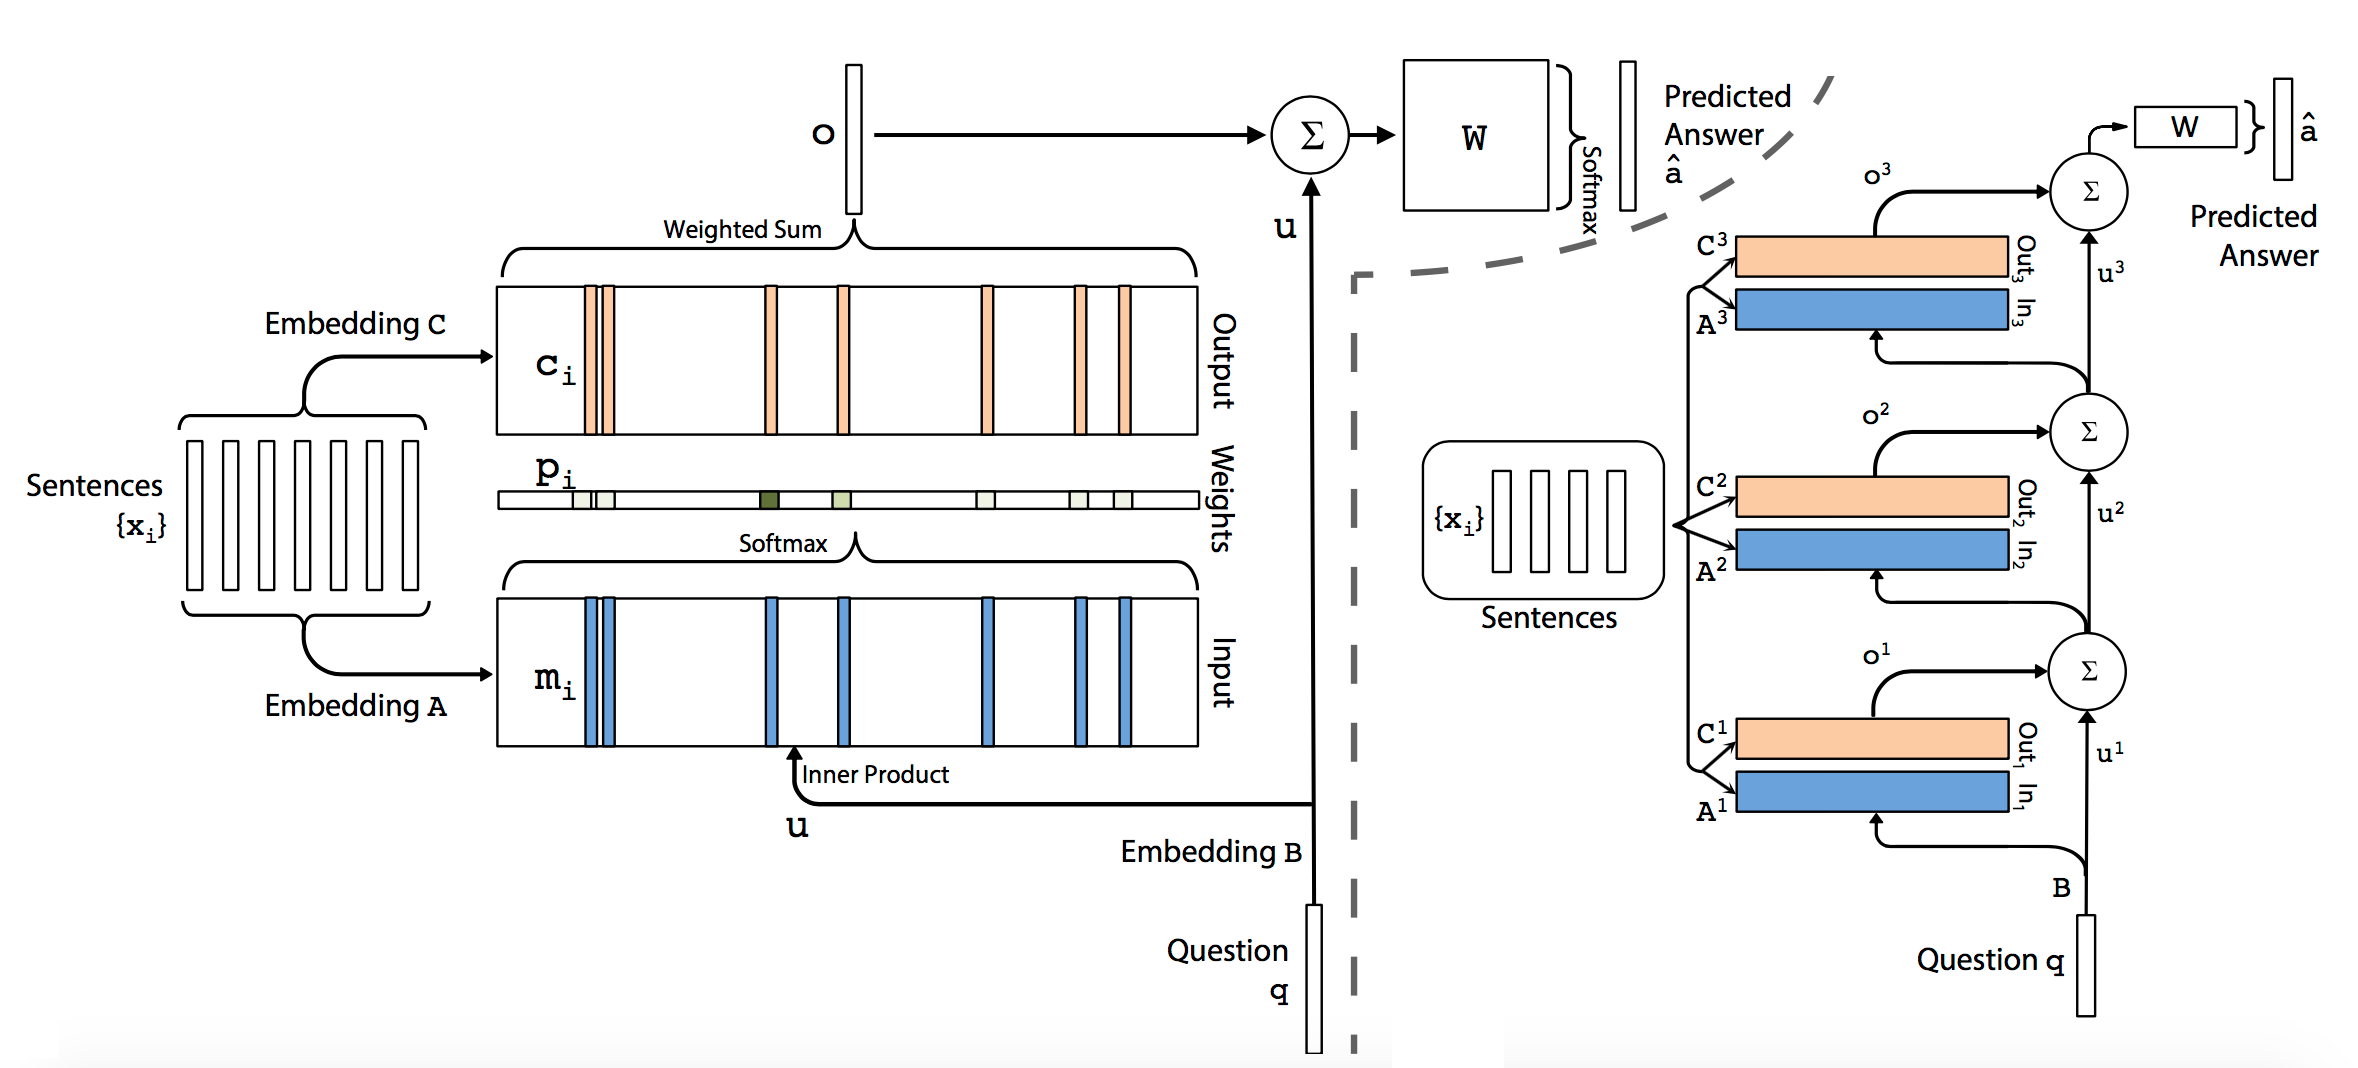
\includegraphics[width=0.7\textwidth]{mem.png}
    \caption{1-Hop and 3-Hop  MeMNetwork}
\end{center}
\end{figure}
\noindent But as one can see on figure 1, we can in fact stack mutliple hop to memory, in this case 3. This would increase performance when dealing with tasks that would require reasoning on more than one fact. In more details, we define the intermediate outputs $o_k$ and $u_k$ by:
\begin{gather*}
o_k  = \sum\limits_{i=1}softmax(u_k^Tm_i) \\
u_{k+1}  = u_k + o_k
\end{gather*} 
\subsection{Parameters Tying}
As mentioned in Sukhbaatar's paper, if using multiple hops to memory yields better results, it also has for consequence to increase significantly the number of parameters. We therefore investigated two different constraints on the embedding matrics $A_i$ and $C_i$, known as parameter tying:
\begin{itemize}
\item \textbf{Adjacent}: $A_{i+1} = C_i$ i.e. the current output embedding is equal to the next input embedding,
\item \textbf{Layer-wise or RNN-like}:  $A_{i+1} = A_i$ and  $C_{i+1} = C_i$ for all $i$
\end{itemize}
When using the RNN-like tying, it is prefered to use define $u_{i+1}$ as a linear transformation of $u_k$, i.e. $u_{i+1} = H u_{i} + o_{i}$. We will compare results using the two different tying methods in the next section.

\section{Experiment}
\subsection{Data and Preprocessing}
[A FAIRE]
- padding with parameters set to 0 for padding
- List Answers
- Reponse similaire dans le train et le test

\subsection{Implementation Details}
\noindent We tested multiple hacks in order to improve performance that we will now detail.
\paragraph{Temporal Encoding}
In order to account for a certain notion of temporality in our baseline model, we weighted word occurences differently based on how close these words were from the question. For the memory network, we add to both the input and output memories, temporal matrices $T_{A_i}$ and $T_{C_i}$ that will be learn during training, and to which we apply the same parameter constraints as $A_i$ and $C_i$. We refer to Temporal Encoding as TE.
 
\paragraph{Position Encoding}
We choose to represent sentence embeddings as the sum of its words' embeddings for simplicity reasons. Indeed, it was then possible to obtain a standard size of each entry in the memory, equal to the hidden embedding size. Nevertheless, this choice could potentially loose information about word position that concatenation would pick up. To avoid this loss of information, we replace the current memory representation:$$m_i = \sum_j Ax_{ij}$$ by $$m_i = \sum_j l_j\cdot A x_{ij}$$ where $\cdot$ corresponds to the element-wise multiplication and $l_j$ is a fixed vector with entries defined by: $$l_kj = (1-\frac{j}{J})-\frac{k}{D}(1-2\frac{j}{J})$$ with $j$ being the indexed of the sentence, $J$ the number of sentences allowed in memory and $D$ the hidden dimension of embeddings. We refer to position encoding as PE.
\paragraph{Linear Start}
Finally, we implemented what Sukhbaatar defines as Linear Start Training (LS). During training, we start by removing the softmax in each memory layer and use validation loss as our trigger. When loss stops decreasing, we add the softmaxes back and continue training. 

\subsection{Results}

In order to compare our results with the ones from Sukhbaatar et al, we decided to adopt the same hyperparameters, i.e.:
\begin{itemize}
\item Capped the memory at 50 sentences,
\item Used an embedding dimension equal to: $d=50$,
\item Train using 100 epochs,
\item Used a learning rate of 0.01 which was halfed every 20 iterations.
\end{itemize}
\noindent We did not use batching (even if we implemented it) because of a rather fast training time. Finally, switching to a GPU took more training time due to a poor level of paralisation.\\

\noindent We now summarise the results of our experiments in the following tables:

\begin{table}[H]
\centering
\label{my-label}
 \resizebox{1\textwidth}{6cm}{
\begin{tabular}{cccccccclclcc}
\multicolumn{1}{l}{}                                                                              & \multicolumn{1}{l}{}                                                                & \multicolumn{1}{l}{}                                                                           & \cellcolor[HTML]{FFCCC9}Best                                                             & \cellcolor[HTML]{ECF4FF}Second Best                                                      & \multicolumn{1}{l}{}                                                                     & \cellcolor[HTML]{67FD9A}\begin{tabular}[c]{@{}c@{}}Unexplainable\\ anomality\end{tabular}   & \multicolumn{1}{l}{}                                                                        &                                                                                                &                                                                                             &                                          &                                                                                                &                                                                                                \\
\multicolumn{1}{l}{}                                                                              & \multicolumn{1}{l}{}                                                                & \multicolumn{1}{l}{}                                                                           & \multicolumn{1}{l}{}                                                                     & \multicolumn{1}{l}{}                                                                     & \multicolumn{1}{l}{}                                                                     & \multicolumn{1}{l}{}                                                                        & \multicolumn{1}{l}{}                                                                        &                                                                                                &                                                                                             &                                          & \multicolumn{1}{l}{}                                                                           & \multicolumn{1}{l}{}                                                                           \\ \cline{3-10} \cline{12-13} 
\multicolumn{1}{l}{}                                                                              & \multicolumn{1}{l|}{}                                                               & \multicolumn{7}{c|}{Jointly Trained}                                                                                                                                                                                                                                                                                                                                                                                                                                                                                                                                                                                                                                         & \multicolumn{1}{c|}{Individually trained}                                                   & \multicolumn{1}{l|}{}                    & \multicolumn{2}{c|}{\begin{tabular}[c]{@{}c@{}}Sukhbaatar et al\\ Jointly Trained\end{tabular}}                                                                                                 \\ \hline
\multicolumn{1}{|c|}{Task}                                                                        & \multicolumn{1}{c|}{\begin{tabular}[c]{@{}c@{}}Count-Based\\ Baseline\end{tabular}} & \multicolumn{1}{c|}{\begin{tabular}[c]{@{}c@{}}3-hop MemNN\\ RNN-Like\\ TE  + PE\end{tabular}} & \multicolumn{1}{c|}{\begin{tabular}[c]{@{}c@{}}1-hop MemNN\\ Adjacent\\ TE\end{tabular}} & \multicolumn{1}{c|}{\begin{tabular}[c]{@{}c@{}}2-hop MemNN\\ Adjacent\\ TE\end{tabular}} & \multicolumn{1}{c|}{\begin{tabular}[c]{@{}c@{}}3-hop MemNN\\ Adjacent\\ TE\end{tabular}} & \multicolumn{1}{c|}{\begin{tabular}[c]{@{}c@{}}2-hop MemNN\\ Adjacent\\ TE+PE\end{tabular}} & \multicolumn{1}{c|}{\begin{tabular}[c]{@{}c@{}}3-hop MemNN\\ Adjacent\\ TE+PE\end{tabular}} & \multicolumn{1}{c|}{\begin{tabular}[c]{@{}c@{}}3-hop MemNN\\ Adjacent\\ TE+PE+LS\end{tabular}} & \multicolumn{1}{c|}{\begin{tabular}[c]{@{}c@{}}3-hop MemNN\\ Adjacent\\ TE+PE\end{tabular}} & \multicolumn{1}{l|}{}                    & \multicolumn{1}{c|}{\begin{tabular}[c]{@{}c@{}}3-hop MemNN\\ Adjacent\\ TE+PE+LS\end{tabular}} & \multicolumn{1}{c|}{\begin{tabular}[c]{@{}c@{}}3-hop MemNN\\ RNN-Like\\ TE+PE+LS\end{tabular}} \\ \cline{1-10} \cline{12-13} 
\multicolumn{1}{|c|}{1}                                                                           & \multicolumn{1}{c|}{0.5}                                                            & \multicolumn{1}{c|}{0.99}                                                                      & \multicolumn{1}{c|}{\cellcolor[HTML]{FFCCC9}{\color[HTML]{333333} 1}}                    & \multicolumn{1}{c|}{0.97}                                                                & \multicolumn{1}{c|}{\cellcolor[HTML]{ECF4FF}0.99}                                        & \multicolumn{1}{c|}{\cellcolor[HTML]{FFCCC9}1}                                              & \multicolumn{1}{c|}{\cellcolor[HTML]{ECF4FF}0.99}                                           & \multicolumn{1}{l|}{}                                                                          & \multicolumn{1}{c|}{\cellcolor[HTML]{FFCCC9}1}                                              & \multicolumn{1}{l|}{}                    & \multicolumn{1}{c|}{0.99}                                                                      & \multicolumn{1}{c|}{0.99}                                                                      \\ \cline{1-1}
\multicolumn{1}{|c|}{2}                                                                           & \multicolumn{1}{c|}{0.4}                                                            & \multicolumn{1}{c|}{\cellcolor[HTML]{ECF4FF}0.79}                                              & \multicolumn{1}{c|}{0.24}                                                                & \multicolumn{1}{c|}{0.25}                                                                & \multicolumn{1}{c|}{0.37}                                                                & \multicolumn{1}{c|}{\cellcolor[HTML]{FFCCC9}0.88}                                           & \multicolumn{1}{c|}{\cellcolor[HTML]{FFFFFF}0.78}                                           & \multicolumn{1}{l|}{}                                                                          & \multicolumn{1}{c|}{0.31}                                                                   & \multicolumn{1}{l|}{}                    & \multicolumn{1}{c|}{0.86}                                                                      & \multicolumn{1}{c|}{0.81}                                                                      \\ \cline{1-1}
\multicolumn{1}{|c|}{3}                                                                           & \multicolumn{1}{c|}{0.26}                                                           & \multicolumn{1}{c|}{0.36}                                                                      & \multicolumn{1}{c|}{0.21}                                                                & \multicolumn{1}{c|}{0.25}                                                                & \multicolumn{1}{c|}{0.21}                                                                & \multicolumn{1}{c|}{\cellcolor[HTML]{ECF4FF}0.65}                                           & \multicolumn{1}{c|}{\cellcolor[HTML]{FFCCC9}0.676}                                          & \multicolumn{1}{l|}{}                                                                          & \multicolumn{1}{c|}{0.33}                                                                   & \multicolumn{1}{l|}{}                    & \multicolumn{1}{c|}{0.76}                                                                      & \multicolumn{1}{c|}{0.68}                                                                      \\ \cline{1-1}
\multicolumn{1}{|c|}{4}                                                                           & \multicolumn{1}{c|}{0.34}                                                           & \multicolumn{1}{c|}{\cellcolor[HTML]{FFCCC9}0.86}                                              & \multicolumn{1}{c|}{0.66}                                                                & \multicolumn{1}{c|}{0.65}                                                                & \multicolumn{1}{c|}{0.66}                                                                & \multicolumn{1}{c|}{0.77}                                                                   & \multicolumn{1}{c|}{\cellcolor[HTML]{ECF4FF}0.81}                                           & \multicolumn{1}{l|}{}                                                                          & \multicolumn{1}{c|}{0.81}                                                                   & \multicolumn{1}{l|}{}                    & \multicolumn{1}{c|}{0.94}                                                                      & \multicolumn{1}{c|}{0.83}                                                                      \\ \cline{1-1}
\multicolumn{1}{|c|}{5}                                                                           & \multicolumn{1}{c|}{0.48}                                                           & \multicolumn{1}{c|}{\cellcolor[HTML]{ECF4FF}0.84}                                              & \multicolumn{1}{c|}{0.83}                                                                & \multicolumn{1}{c|}{0.82}                                                                & \multicolumn{1}{c|}{0.83}                                                                & \multicolumn{1}{c|}{\cellcolor[HTML]{ECF4FF}0.84}                                           & \multicolumn{1}{c|}{\cellcolor[HTML]{FFCCC9}0.96}                                           & \multicolumn{1}{l|}{}                                                                          & \multicolumn{1}{c|}{\cellcolor[HTML]{ECF4FF}0.84}                                           & \multicolumn{1}{l|}{}                    & \multicolumn{1}{c|}{0.85}                                                                      & \multicolumn{1}{c|}{0.87}                                                                      \\ \cline{1-1}
\multicolumn{1}{|c|}{6}                                                                           & \multicolumn{1}{c|}{0.5}                                                            & \multicolumn{1}{c|}{\cellcolor[HTML]{ECF4FF}0.97}                                              & \multicolumn{1}{c|}{0.76}                                                                & \multicolumn{1}{c|}{0.93}                                                                & \multicolumn{1}{c|}{0.93}                                                                & \multicolumn{1}{c|}{\cellcolor[HTML]{FFCCC9}0.99}                                           & \multicolumn{1}{c|}{0.83}                                                                   & \multicolumn{1}{l|}{}                                                                          & \multicolumn{1}{c|}{0.92}                                                                   & \multicolumn{1}{l|}{}                    & \multicolumn{1}{c|}{0.97}                                                                      & \multicolumn{1}{c|}{0.98}                                                                      \\ \cline{1-1}
\multicolumn{1}{|c|}{7}                                                                           & \multicolumn{1}{c|}{0.49}                                                           & \multicolumn{1}{c|}{0.85}                                                                      & \multicolumn{1}{c|}{0.84}                                                                & \multicolumn{1}{c|}{0.82}                                                                & \multicolumn{1}{c|}{0.86}                                                                & \multicolumn{1}{c|}{\cellcolor[HTML]{ECF4FF}0.87}                                           & \multicolumn{1}{c|}{\cellcolor[HTML]{FFCCC9}0.89}                                           & \multicolumn{1}{l|}{}                                                                          & \multicolumn{1}{c|}{0.79}                                                                   & \multicolumn{1}{l|}{}                    & \multicolumn{1}{c|}{0.82}                                                                      & \multicolumn{1}{c|}{0.90}                                                                      \\ \cline{1-1}
\multicolumn{1}{|c|}{8}                                                                           & \multicolumn{1}{c|}{0}                                                              & \multicolumn{1}{c|}{\cellcolor[HTML]{ECF4FF}0.90}                                              & \multicolumn{1}{c|}{0.89}                                                                & \multicolumn{1}{c|}{0.87}                                                                & \multicolumn{1}{c|}{\cellcolor[HTML]{ECF4FF}0.90}                                        & \multicolumn{1}{c|}{\cellcolor[HTML]{ECF4FF}0.90}                                           & \multicolumn{1}{c|}{\cellcolor[HTML]{FFCCC9}0.98}                                           & \multicolumn{1}{l|}{}                                                                          & \multicolumn{1}{c|}{0.88}                                                                   & \multicolumn{1}{l|}{}                    & \multicolumn{1}{c|}{0.90}                                                                      & \multicolumn{1}{c|}{0.94}                                                                      \\ \cline{1-1}
\multicolumn{1}{|c|}{9}                                                                           & \multicolumn{1}{c|}{0.64}                                                           & \multicolumn{1}{c|}{0.95}                                                                      & \multicolumn{1}{c|}{0.80}                                                                & \multicolumn{1}{c|}{\cellcolor[HTML]{ECF4FF}0.96}                                        & \multicolumn{1}{c|}{0.95}                                                                & \multicolumn{1}{c|}{\cellcolor[HTML]{FFCCC9}0.99}                                           & \multicolumn{1}{c|}{0.94}                                                                   & \multicolumn{1}{l|}{}                                                                          & \multicolumn{1}{c|}{0.76}                                                                   & \multicolumn{1}{l|}{}                    & \multicolumn{1}{c|}{0.97}                                                                      & \multicolumn{1}{c|}{0.99}                                                                      \\ \cline{1-1}
\multicolumn{1}{|c|}{10}                                                                          & \multicolumn{1}{c|}{0.44}                                                           & \multicolumn{1}{c|}{0.81}                                                                      & \multicolumn{1}{c|}{0.68}                                                                & \multicolumn{1}{c|}{\cellcolor[HTML]{ECF4FF}0.90}                                        & \multicolumn{1}{c|}{0.87}                                                                & \multicolumn{1}{c|}{\cellcolor[HTML]{FFCCC9}0.95}                                           & \multicolumn{1}{c|}{\cellcolor[HTML]{ECF4FF}0.90}                                           & \multicolumn{1}{l|}{}                                                                          & \multicolumn{1}{c|}{0.66}                                                                   & \multicolumn{1}{l|}{}                    & \multicolumn{1}{c|}{0.94}                                                                      & \multicolumn{1}{c|}{0.97}                                                                      \\ \cline{1-1}
\multicolumn{1}{|c|}{11}                                                                          & \multicolumn{1}{c|}{0.63}                                                           & \multicolumn{1}{c|}{\cellcolor[HTML]{ECF4FF}0.95}                                              & \multicolumn{1}{c|}{0.91}                                                                & \multicolumn{1}{c|}{0.90}                                                                & \multicolumn{1}{c|}{0.91}                                                                & \multicolumn{1}{c|}{\cellcolor[HTML]{FFCCC9}0.97}                                           & \multicolumn{1}{c|}{0.93}                                                                   & \multicolumn{1}{l|}{}                                                                          & \multicolumn{1}{c|}{0.86}                                                                   & \multicolumn{1}{l|}{}                    & \multicolumn{1}{c|}{0.99}                                                                      & \multicolumn{1}{c|}{0.97}                                                                      \\ \cline{1-1}
\multicolumn{1}{|c|}{12}                                                                          & \multicolumn{1}{c|}{0.60}                                                           & \multicolumn{1}{c|}{\cellcolor[HTML]{ECF4FF}0.99}                                              & \multicolumn{1}{c|}{1}                                                                   & \multicolumn{1}{c|}{0.97}                                                                & \multicolumn{1}{c|}{\cellcolor[HTML]{FFCCC9}1}                                           & \multicolumn{1}{c|}{\cellcolor[HTML]{FFCCC9}1}                                              & \multicolumn{1}{c|}{0.93}                                                                   & \multicolumn{1}{l|}{}                                                                          & \multicolumn{1}{c|}{\cellcolor[HTML]{FFCCC9}1}                                              & \multicolumn{1}{l|}{}                    & \multicolumn{1}{c|}{0.99}                                                                      & \multicolumn{1}{c|}{1}                                                                         \\ \cline{1-1}
\multicolumn{1}{|c|}{13}                                                                          & \multicolumn{1}{c|}{0.68}                                                           & \multicolumn{1}{c|}{\cellcolor[HTML]{FFCCC9}0.99}                                              & \multicolumn{1}{c|}{\cellcolor[HTML]{ECF4FF}0.94}                                        & \multicolumn{1}{c|}{0.87}                                                                & \multicolumn{1}{c|}{\cellcolor[HTML]{ECF4FF}0.94}                                        & \multicolumn{1}{c|}{\cellcolor[HTML]{FFCCC9}0.99}                                           & \multicolumn{1}{c|}{0.93}                                                                   & \multicolumn{1}{l|}{}                                                                          & \multicolumn{1}{c|}{0.92}                                                                   & \multicolumn{1}{l|}{}                    & \multicolumn{1}{c|}{0.98}                                                                      & \multicolumn{1}{c|}{0.99}                                                                      \\ \cline{1-1}
\multicolumn{1}{|c|}{14}                                                                          & \multicolumn{1}{c|}{0.29}                                                           & \multicolumn{1}{c|}{0.79}                                                                      & \multicolumn{1}{c|}{0.65}                                                                & \multicolumn{1}{c|}{\cellcolor[HTML]{FFCCC9}0.94}                                        & \multicolumn{1}{c|}{0.84}                                                                & \multicolumn{1}{c|}{\cellcolor[HTML]{FFCCC9}0.94}                                           & \multicolumn{1}{c|}{0.84}                                                                   & \multicolumn{1}{l|}{}                                                                          & \multicolumn{1}{c|}{\cellcolor[HTML]{ECF4FF}0.87}                                           & \multicolumn{1}{l|}{}                    & \multicolumn{1}{c|}{0.92}                                                                      & \multicolumn{1}{c|}{0.98}                                                                      \\ \cline{1-1}
\multicolumn{1}{|c|}{15}                                                                          & \multicolumn{1}{c|}{0.14}                                                           & \multicolumn{1}{c|}{\cellcolor[HTML]{FFCCC9}0.55}                                              & \multicolumn{1}{c|}{0.41}                                                                & \multicolumn{1}{c|}{0.33}                                                                & \multicolumn{1}{c|}{0.40}                                                                & \multicolumn{1}{c|}{0.38}                                                                   & \multicolumn{1}{c|}{0.42}                                                                   & \multicolumn{1}{l|}{}                                                                          & \multicolumn{1}{c|}{\cellcolor[HTML]{ECF4FF}0.50}                                           & \multicolumn{1}{l|}{}                    & \multicolumn{1}{c|}{\cellcolor[HTML]{67FD9A}1}                                                 & \multicolumn{1}{c|}{0.98}                                                                      \\ \cline{1-1}
\multicolumn{1}{|c|}{16}                                                                          & \multicolumn{1}{c|}{0.52}                                                           & \multicolumn{1}{c|}{\cellcolor[HTML]{ECF4FF}0.50}                                              & \multicolumn{1}{c|}{\cellcolor[HTML]{FFCCC9}0.51}                                        & \multicolumn{1}{c|}{0.47}                                                                & \multicolumn{1}{c|}{0.49}                                                                & \multicolumn{1}{c|}{0.49}                                                                   & \multicolumn{1}{c|}{0.45}                                                                   & \multicolumn{1}{l|}{}                                                                          & \multicolumn{1}{c|}{0.49}                                                                   & \multicolumn{1}{l|}{}                    & \multicolumn{1}{c|}{\cellcolor[HTML]{67FD9A}0.96}                                              & \multicolumn{1}{c|}{0.49}                                                                      \\ \cline{1-1}
\multicolumn{1}{|c|}{17}                                                                          & \multicolumn{1}{c|}{0.48}                                                           & \multicolumn{1}{c|}{0.56}                                                                      & \multicolumn{1}{c|}{0.49}                                                                & \multicolumn{1}{c|}{0.52}                                                                & \multicolumn{1}{c|}{\cellcolor[HTML]{FFCCC9}0.59}                                        & \multicolumn{1}{c|}{0.55}                                                                   & \multicolumn{1}{c|}{0.54}                                                                   & \multicolumn{1}{l|}{}                                                                          & \multicolumn{1}{c|}{\cellcolor[HTML]{ECF4FF}0.57}                                           & \multicolumn{1}{l|}{}                    & \multicolumn{1}{c|}{0.56}                                                                      & \multicolumn{1}{c|}{0.58}                                                                      \\ \cline{1-1}
\multicolumn{1}{|c|}{18}                                                                          & \multicolumn{1}{c|}{0.53}                                                           & \multicolumn{1}{c|}{0.79}                                                                      & \multicolumn{1}{c|}{0.48}                                                                & \multicolumn{1}{c|}{0.49}                                                                & \multicolumn{1}{c|}{0.47}                                                                & \multicolumn{1}{c|}{0.55}                                                                   & \multicolumn{1}{c|}{\cellcolor[HTML]{ECF4FF}0.90}                                           & \multicolumn{1}{l|}{}                                                                          & \multicolumn{1}{c|}{\cellcolor[HTML]{FFCCC9}0.92}                                           & \multicolumn{1}{l|}{}                    & \multicolumn{1}{c|}{0.90}                                                                      & \multicolumn{1}{c|}{0.91}                                                                      \\ \cline{1-1}
\multicolumn{1}{|c|}{19}                                                                          & \multicolumn{1}{c|}{0}                                                              & \multicolumn{1}{c|}{0.01}                                                                      & \multicolumn{1}{c|}{0.09}                                                                & \multicolumn{1}{c|}{0.08}                                                                & \multicolumn{1}{c|}{0.11}                                                                & \multicolumn{1}{c|}{\cellcolor[HTML]{ECF4FF}0.13}                                           & \multicolumn{1}{c|}{\cellcolor[HTML]{FFCCC9}0.18}                                           & \multicolumn{1}{l|}{}                                                                          & \multicolumn{1}{c|}{0.11}                                                                   & \multicolumn{1}{l|}{}                    & \multicolumn{1}{c|}{0.1}                                                                       & \multicolumn{1}{c|}{0.09}                                                                      \\ \cline{1-1}
\multicolumn{1}{|c|}{20}                                                                          & \multicolumn{1}{c|}{0.52}                                                           & \multicolumn{1}{c|}{\cellcolor[HTML]{FFCCC9}0.97}                                              & \multicolumn{1}{c|}{0.92}                                                                & \multicolumn{1}{c|}{0.92}                                                                & \multicolumn{1}{c|}{0.92}                                                                & \multicolumn{1}{c|}{\cellcolor[HTML]{ECF4FF}0.95}                                           & \multicolumn{1}{c|}{0.92}                                                                   & \multicolumn{1}{l|}{}                                                                          & \multicolumn{1}{c|}{0.92}                                                                   & \multicolumn{1}{l|}{}                    & \multicolumn{1}{c|}{1}                                                                         & \multicolumn{1}{c|}{0.99}                                                                      \\ \cline{1-10} \cline{12-13} 
\multicolumn{1}{|c|}{TOTAL}                                                                       & \multicolumn{1}{c|}{0.42}                                                           & \multicolumn{1}{c|}{0.77}                                                                      & \multicolumn{1}{c|}{0.67}                                                                & \multicolumn{1}{c|}{0.69}                                                                & \multicolumn{1}{c|}{0.71}                                                                & \multicolumn{1}{c|}{\cellcolor[HTML]{FFCCC9}0.79}                                           & \multicolumn{1}{c|}{\cellcolor[HTML]{ECF4FF}0.78}                                           & \multicolumn{1}{l|}{}                                                                          & \multicolumn{1}{c|}{0.72}                                                                   & \multicolumn{1}{l|}{}                    & \multicolumn{1}{c|}{0.87}                                                                      & \multicolumn{1}{c|}{0.85}                                                                      \\ \cline{1-10} \cline{12-13} 
\multicolumn{1}{|c|}{\begin{tabular}[c]{@{}c@{}}Failed Tasks\\ (Acc \textless 0.95)\end{tabular}} & \multicolumn{1}{c|}{20}                                                             & \multicolumn{1}{c|}{13}                                                                        & \multicolumn{1}{c|}{20}                                                                  & \multicolumn{1}{c|}{17}                                                                  & \multicolumn{1}{c|}{17}                                                                  & \multicolumn{1}{c|}{12}                                                                     & \multicolumn{1}{c|}{17}                                                                     & \multicolumn{1}{c|}{}                                                                          & \multicolumn{1}{c|}{18}                                                                     & \multicolumn{1}{l|}{\multirow{-23}{*}{}} & \multicolumn{1}{c|}{11}                                                                        & \multicolumn{1}{c|}{10}                                                                        \\ \cline{1-10} \cline{12-13} 
\end{tabular}
}
\caption{Accuracy Results on held-out test data}
\end{table}

The first obvious 
\section{Future Work}
\subsection{Application to the MCTest dataset}
Results on the bAbi dataset were encouraging but have to be put in perspective. Indeed, the size and quality of the stories, the number of word in the vocabulary, the fact that answers appear both in the training and test data make it a rather easy dataset to work on. In order to challenge the algorithm, we wanted to test it on the MCTest dataset. This dataset contains 660 stories and multiple choice questions with sentences answers. For instance:
\begin{framed}
\begin{center}
Q:  What did James do after he ordered the fries?\\
A) went to the grocery store\\
B) went home without paying\\
C) ate them\\
D) made up his mind to be a better turle\\
\end{center}
\end{framed}
\noindent With these types of question, we can not use the same trick as for the bAby, i.e. use a final linear model and softmax layer to predict a distribution over possible answers that appeared in the training set. What we propose instead is to introduce a matrix $D$ used to embed the answers and store them in $a_1, a_2, a_3$ and $a_4$ and use the last intermediate output $u_K = u_{K-1} + o_{K-1}$ (where $K$ is the number of hops) to evaluate the cosine similarity with the $a_i$'s:
$$sim(u_K,a_i) = \frac{u_K \cdot a_i}{||u_K||\,||a_i||}.$$ We can then normalise the scores using a softmax transformation and use regular NNL loss to train the model.

\subsection{Dynamic Memory Networks}
[A FAIRE]
\section{Conclusion}
[A FAIRE]
\vskip 0.2in
\bibliography{sample}

\end{document}